\begin{document}
	
	\section{Pipeline Description}
	
	
	
	The aim of this thesis works is to develop a pipeline for identification of GGO and CS areas in chest CT scans of patients affected by COVID-19, that aims to have the following characteristics:   
	\begin{itemize}
		\item  \textbf{Fully Automated: } to remove the dependency from an external operator, and so the subjectivity of the segmentation; 
		
		\item \textbf{Fast: } in order to compete with certified software and to provides a segmentation in few minutes.
	\end{itemize}

	Before going in deep and starting the description, I will define this kind of regions. 	
	Austin in ~\cite{ART:Austin} has defined the Ground Glass Opacities as an "\emph{Hazy increased attenuation of lung, but with preservation of bronchial and vascular margins; caused by partial filling of air spaces, interstitial thickening, partial collapse of alveoli,normal expiration, or increased capillary blood volume.}", which is different from consolidation in which bronchovascular margins are obscured. An example of these areas in displayed in \figurename\,\ref{fig:GGO}.

 %The whole pipeline was developed and tested on CT scans kindly provided by Sant'Orsola Hospital. Also the public datasets were used as benchmark. The used datasets are manually annotated; the provided labels are used to check the pipeline performances.\\ During the pipeline developing we have to takes into account that the infection regions may have different patterns according to the stage of the disease or recovery, as we can see in \figurename\,\ref{fig:GGO-Spatial}, and usually these patterns are spatially disconnected; so we have decided to use a pixel classification technique.\\
	
	
	\begin{figure}[h!]
		\centering
			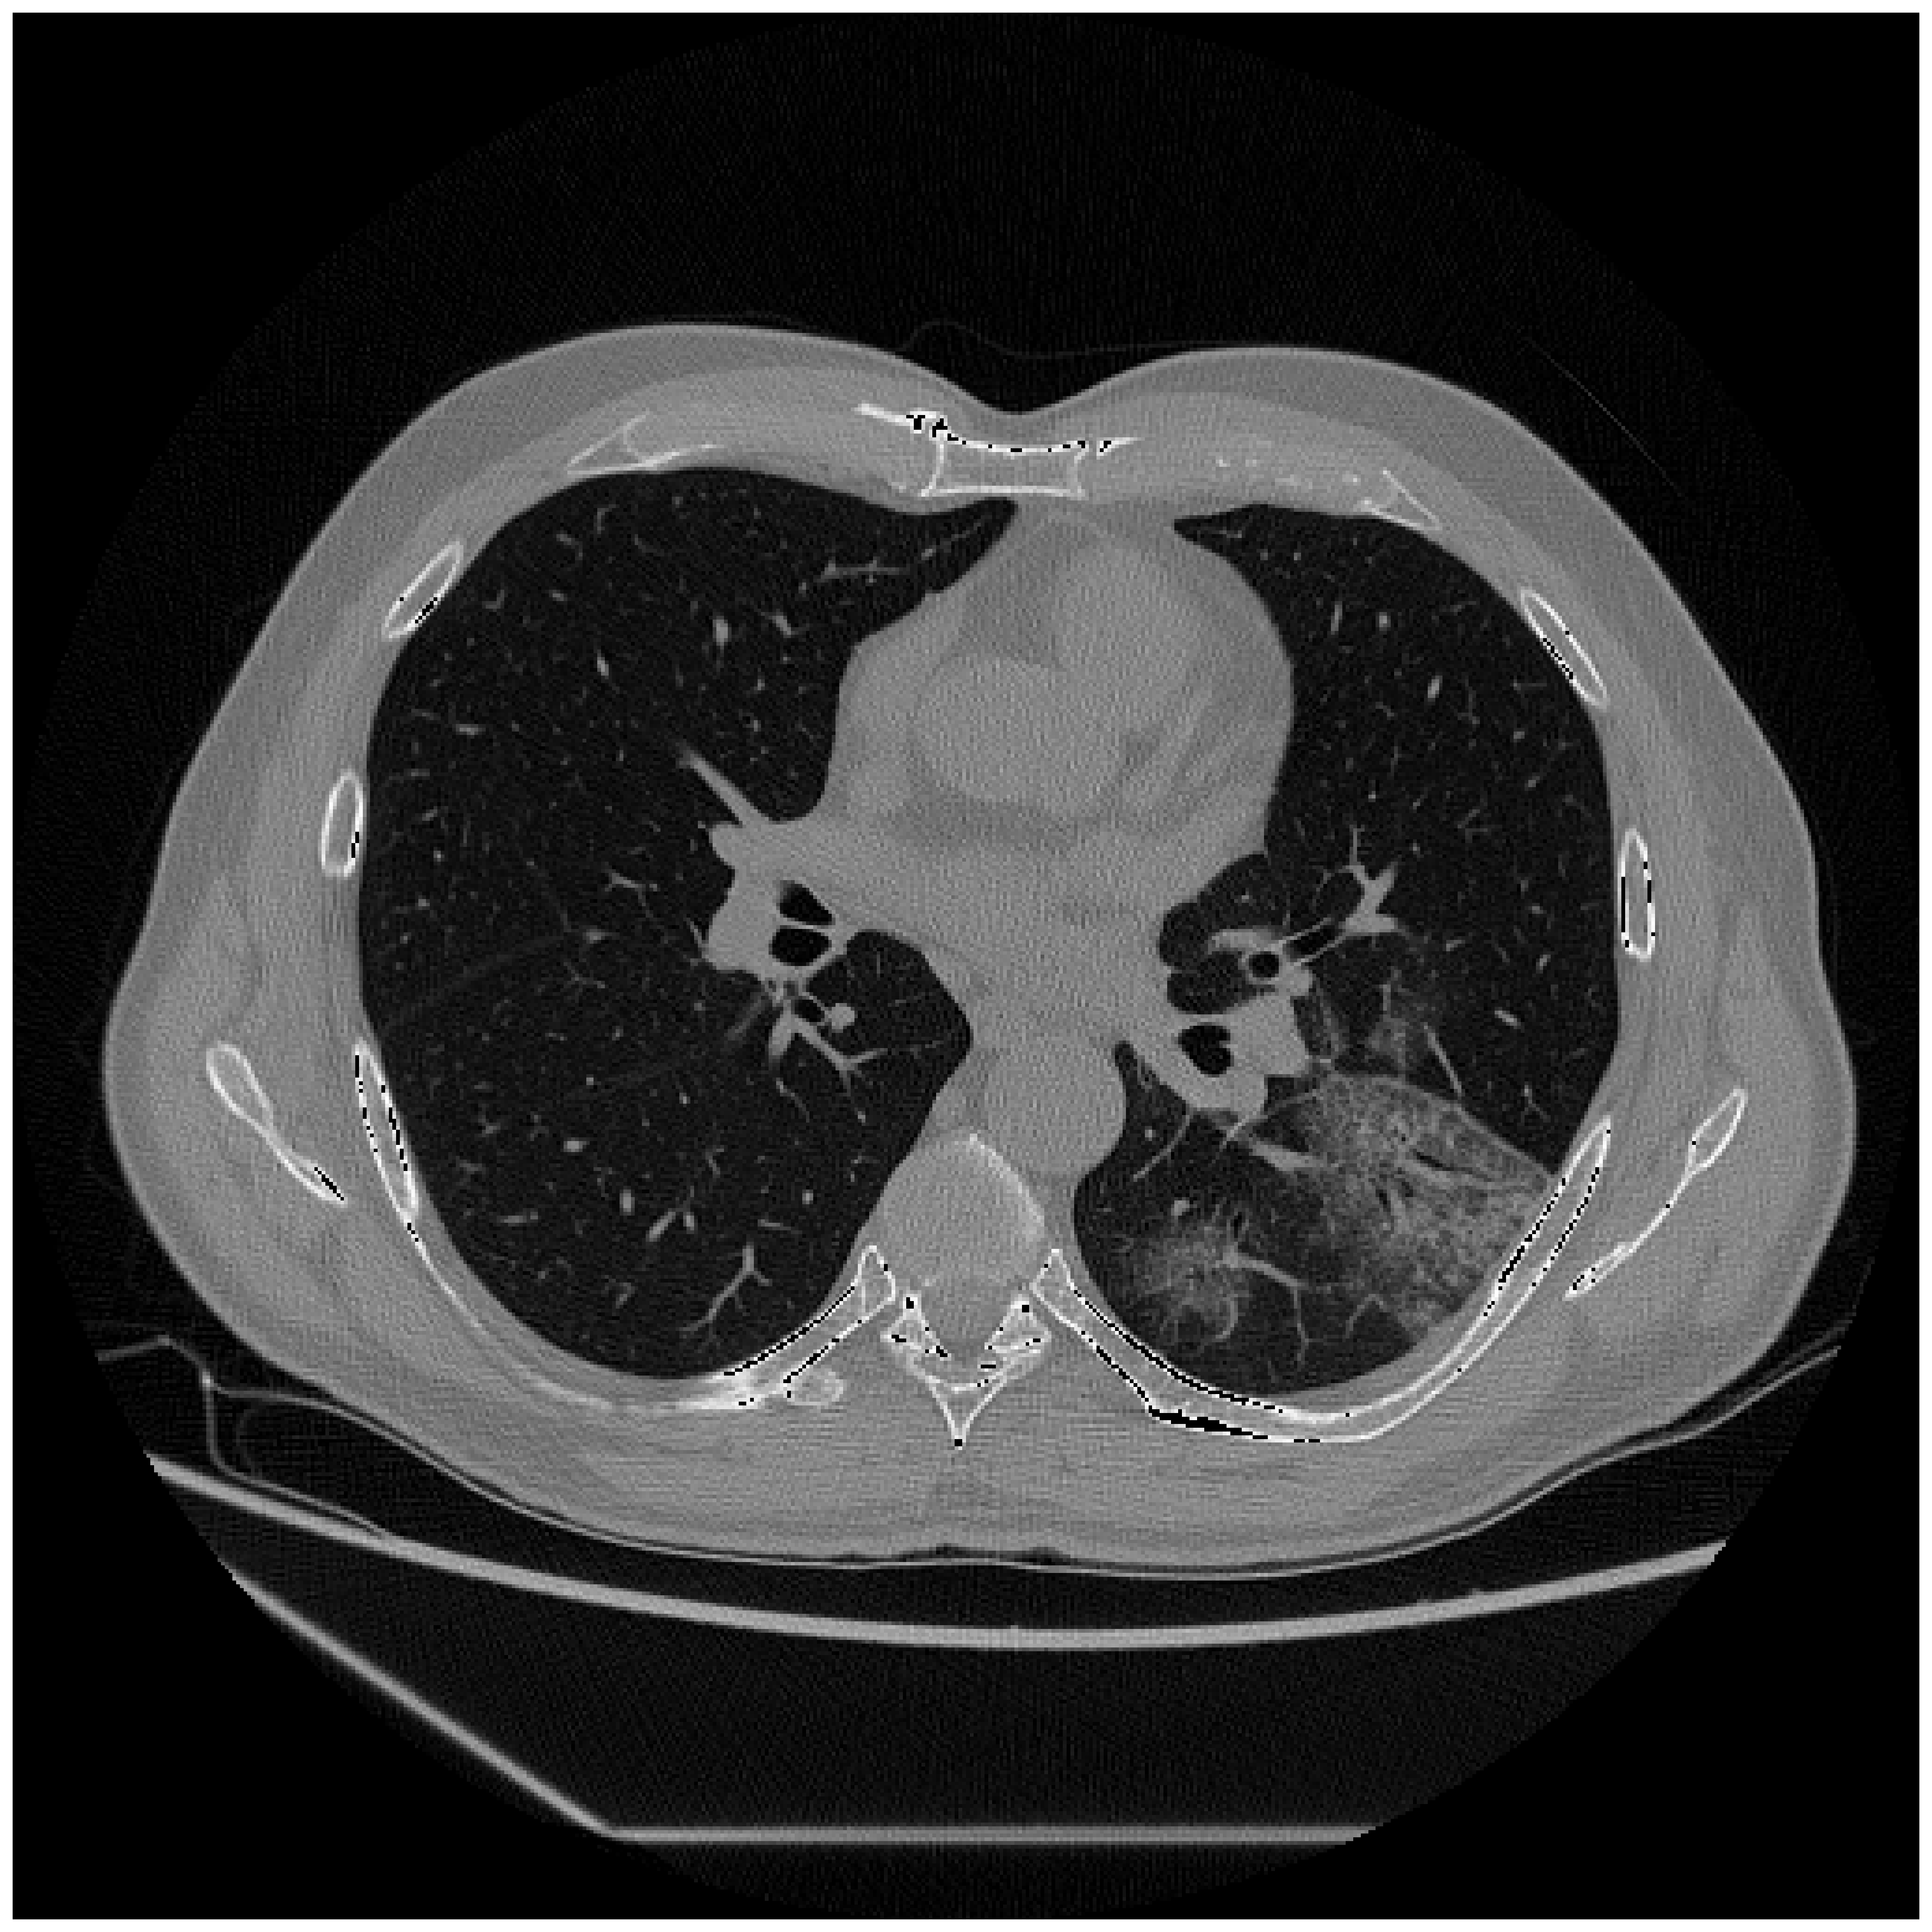
\includegraphics[scale=.5]{GGO.png}
		\caption{Chest CT image of a patient affected by COVID-19. We can see GGO and CS on the right lung. We can appreciate how the different structures, like lesions, are identified by similar color, so the basic segmentation idea was to group voxel by color similarity.}
	\label{fig:GGO}
	\end{figure}

	The segmentation is based on an unsupervised technique, so doesn't requires to provide the expected outcomes.
	As we can see in the chest CT scan in \figurename\,\ref{fig:GGO} the different structure are characterized by similar gray level: the basic idea was to use the color quantization for medical image segmentation, grouping voxel based on color similarity, and  assign  to each tissue a characteristic color. This can be done since in CT scan exist a relationship between the tissue in the voxel and the Gray Level used to display it, given by the Hounsfiend Units(eq\,\ref{eq:HU}), so colors are proportional to HU, which are defined as a linear transformation of the linear attenuation coefficient($\mu$).
		
	Color quantization and the properties of digital images allows to consider also other properties of the image besides the single voxel intensity:
	As I've said before, in digital image processing, images are represented with a 3D tensor, in which the first two dimensions represent the height and width of the image  and the last one the number of channels. 
	In this work we have used the different channels to takes in account different properties, exploited by the application of suitable filters on the original scan. This allow us to consider also neighboring voxels, that is really suitable for the segmentation since the  lesions areas involves many closest voxels, not only a single one. 
	
	Once we have build the color space, we have to found the characteristic color of each tissue under study, which is represented by a centroids in the color space. In order to perform this task and achieve the centroids estimation, a simple k-means clustering was used, since it provides a suitable segmentation with good time performances and it is efficiently implemented for multi-channel images in \textsf{OpenCV}~\cite{OpenCV}.
	 
	K-means clustering requires a prior knowledge about the number of cluster, which in our case is given by the anatomical structure of the lung; so we can consider a different cluster for each anatomical structure.
	Once we have estimated the centroids for each tissue, we have used them for the actual segmentation, by assign each voxel to the cluster of the closest centroids: in this way the estimation step, that we will call "train", needs to be performed only once, so can be time expansive since is not involved in the actual segmentation.\\
	
\end{document}